\section{Introduction}
\label{sec: introduction}

\IEEEPARstart{W}{ith} the great success of deep learning in computer vision, this decade has witnessed an explosion of deep learning based computer vision applications. Because of the huge computational resource consumption for deep learning applications (e.g., inferring an image on VGG19~\cite{VGG19} requires 20 GFLOPs of GPU resource), in today's computer vision applications, users usually have to upload the input images to the central cloud service providers (e.g., SenseTime, Baidu Vision and Google Vision, etc.), leading to a significant upload traffic load. For example, a picture taken by a cellphone at the resolution of $3968 \times 2976$ when saved as JPEG format at the default compression quality level, has a size up to 3MB. %% \\

To reduce the upload traffic load, it is straightforward that an image should be compressed before one uploads it. Though JPEG has been used as the {\em de facto} image compression and encapsulation method, its performance for the deep computer vision models is not satisfactory, because JPEG was originally designed for the Human-Visual System. Liu et al.~\cite{DeepN-JPEG} showed that by redesigning the \emph{quantization table} in the default JPEG configuration, by retraining it on the original dataset, one can compress an image to a smaller version while maintaining the inference accuracy for a fixed deep computer vision algorithm. We then raise an intuitive question: to make it practically useful, can we improve the JPEG configuration adaptively for different cloud computer vision services, without any pre-knowledge of the original model and dataset? %% \\

Our answer to this question is a new learning-based compression methodology for today's cloud computer vision services. We tackle the following challenges in our design. %% \\

\begin{itemize}
\item \textbf{Lack of information about the cloud computer vision models.} Different from the studies ~\cite{DeepN-JPEG,torfason2018towards,gueguen2018faster}, in which the computer vision models are available so that one can adjust the JPEG configuration according to the model structure or retrain the parameters in it, e.g., one can greedily search a gradient descent to reach an optimal compression quality level in JPEG. In our study, however, the details of the online cloud computer vision model are inaccessible. %% \\

\item \textbf{Different cloud computer vision models need different JPEG configurations.} As an adaptive JPEG configuration solution, we target to provide a solution that is adaptive to different cloud computer vision services, i.e., it can \emph{generate} JPEG configuration for different models. However, today's cloud computer vision algorithms, based one deep and convolutional computations, are quite hard to understand. The same compression quality level could lead to a totally different accuracy performance. Some examples are shown in Figure \ref{fig: compress_accuracy}, picture 1a and 1b, 2a and 2b are visually similar for human beings, but the deep learning models give different inference results, only because they are compressed at different quality levels. And such a relationship is not apparent, e.g., picture 3b is highly compressed and looks destroyed comparing to picture 3a, but the deep learning model can still recognize it. This phenomenon is also presented in~\cite{delac2005effects} and commonly seen in adversarial neural network researches~\cite{yuan2019adversarial, evtimov2018robust}. %% \\

\item \textbf{Lack of well-labeled training data.} In our problem, one is not provided the well-labeled data on which image should be compressed to which quality level, as in conventional supervised deep learning tasks. In practice, such an image compression module is usually utilized in an online manner, and the solution has to learn from the images it uploads automatically. 
\end{itemize} 

\begin{figure*}[htbp]
%	\begin{tabular}{cc}
	\begin{minipage}{0.5\linewidth}
		\centerline{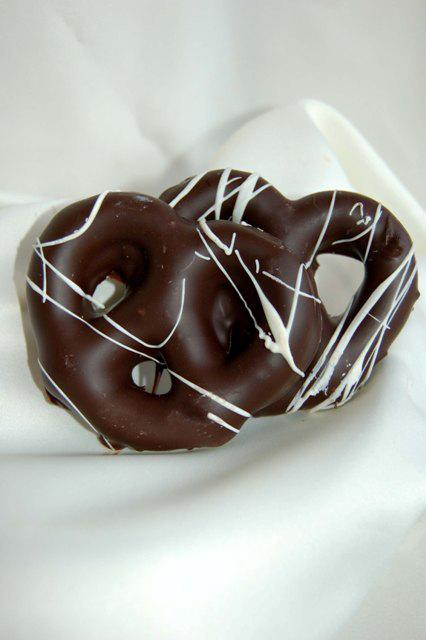
\includegraphics[width=6.0cm, trim=0 150 0 150, clip]{figures/donut_q75.jpeg}}
		\centerline{(1a) Q=75}
%		\centerline{Face++ prediction=["donut"]}
		\centerline{Face++ prediction \ = \ ["donut"]}
		\vspace{0.4cm}
	\end{minipage}
	\hfill
	\begin{minipage}{0.5\linewidth}
		\centerline{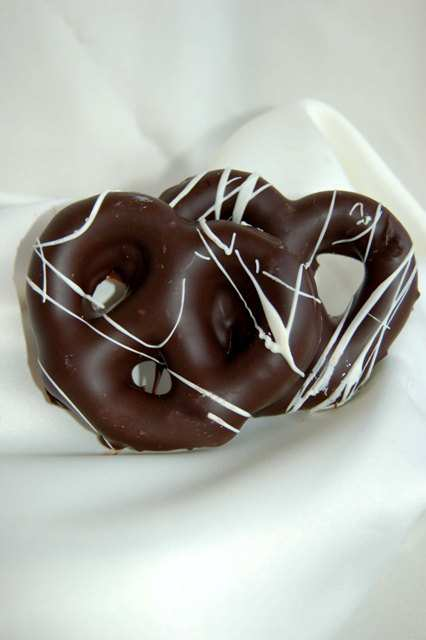
\includegraphics[width=6.0cm, trim=0 150 0 150, clip]{figures/donut_q55.jpeg}}
		\centerline{(1b) Q=55}
%		\centerline{Face++ prediction=[]}
		\centerline{Face++ prediction \ = \ ["biscuit"]}
		\vspace{0.4cm}
	\end{minipage}
	\vfill	
	\begin{minipage}{0.5\linewidth}
		\centerline{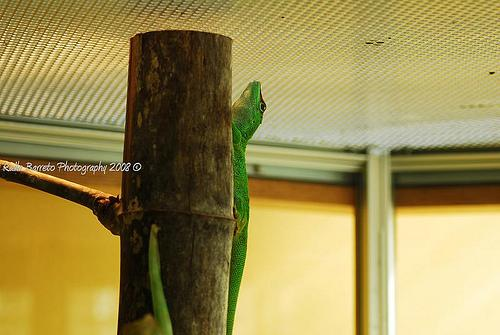
\includegraphics[width=6.0cm, trim=0 0 0 0]{figures/chameleon_q75.jpeg}}
		\centerline{(2a) Q=75}
% 		\centerline{\quad Baidu prediction=["chameleon"]}
		\centerline{Baidu prediction \ = \ ["chameleon"]}
		\vspace{0.4cm}
	\end{minipage}
	\hfill
	\begin{minipage}{0.5\linewidth}
		\centerline{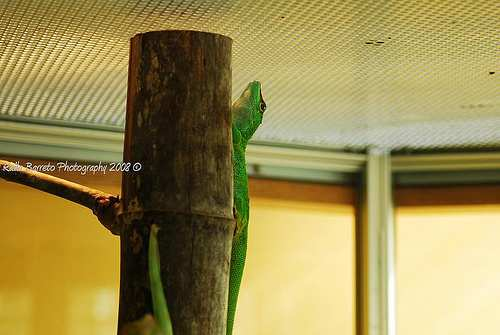
\includegraphics[width=6.0cm, trim=0 0 0 0]{figures/chameleon_q55.jpeg}}
		\centerline{(2b) Q=55}
% 		\centerline{\qquad Baidu prediction=["electric fan"]}
 		\centerline{Baidu prediction \ = \ ["electric fan"]}
 		\vspace{0.4cm}
	\end{minipage}
	\vfill
	\begin{minipage}{0.5\linewidth}
		\centerline{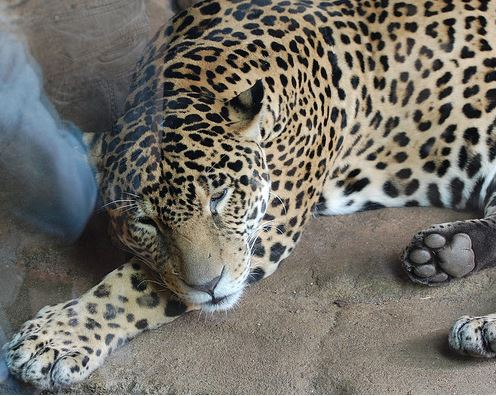
\includegraphics[width=6.0cm, trim=0 0 0 0, clip]{figures/tiger_highq.jpeg}}
		\centerline{(3a) Q=75}
%		\centerline{Baidu prediction=["leopard"]}
		\centerline{Baidu prediction \ = \ ["leopard"]}
		\vspace{0.3cm}
	\end{minipage}
	\hfill
	\begin{minipage}{0.5\linewidth}
		\centerline{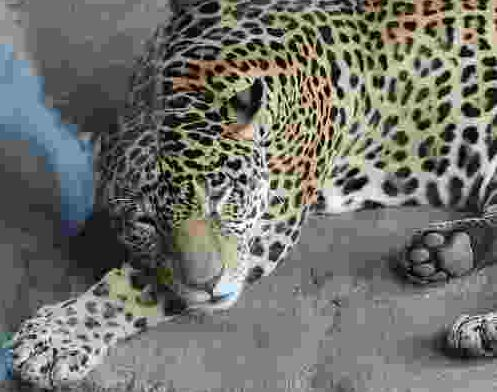
\includegraphics[width=6.0cm, trim=0 0 0 0, clip]{figures/tiger_lowq.jpeg}}
		\centerline{(3b) Q=5}
%		\centerline{Baidu prediction=["leopard"]}
		\centerline{Baidu prediction \ = \ ["leopard"]}
		\vspace{0.3cm}
	\end{minipage}
%	\end{tabular}
	\caption{The prediction of a deep learning model is not completely related to the input image's quality, making it difficult to use a fixed compression quality for all images. For image 1a, 1b and 2a, 2b, minor changes cause different predictions though they are visually similar; for image 3a and 3b, the cloud model still output correct label from a severely compressed image though they look very different}
	\label{fig: compress_accuracy}
%	\vspace{-0.1cm}
\end{figure*}

To address the above challenges, we present a reinforcement learning (RL) based solution, AdaCompress, to choose the proper compression quality level for an image to a computer vision model on the cloud, in an online manner. We open-sourced\footnote{\url{https://github.com/hosea1008/AdaCompress}} our JPEG configuration module that works with today's cloud computing vision APIs upon acceptance of this paper \cite{2019adacompress}. In particular, our contributions are summarized as follows: %% \\

\begin{itemize} \item First, we design an interactive training environment that can be applied to different computer vision cloud services at different times, then we propose a Deep Q-learning Network based agent to evaluate and predict the performance of a compression quality level on an input image. In real-world application scenarios, this agent can be highly efficient to run on today's edge infrastructures (e.g., Google edge TPU \cite{google-tpu}, Huawei Atlas 500 edge station \cite{huawei-atlas500}).
	
	\item Second, we build up a reinforcement learning framework to train the agent in the above environment. The agent can learn to choose a proper compression quality level for an input image after iteratively interacting with the environment by feeding the carefully designed reward comprehensively considering accuracy and data size into it. To make the solution adaptive to the changing input images, we propose an explore-exploit mechanism to adapt the agent to different ``scenery'' online. After deploying the agent, an inference-estimate-retrain mechanism is designed to restart the training procedure once the scenery changes and the existing running agent cannot guarantee stable accuracy performance. 
	
	\item Finally, we provide analysis and insights on our design. We analyze the Q network's behavior by introducing Grad-Cam ~\cite{grad-cam}, explain why the Q network chooses a specific compression quality level and provide some general patterns. Generally speaking, images that contain large smooth areas are more sensitive to compression, while the images with complex textures are more robust to compression when shown to deep learning models. We evaluate our system on some most popular cloud deep learning services, including Amazon Rekognition~\cite{amazon_rekognition}, Face++~\cite{face++_service} and Baidu Vision~\cite{baidu_vision}, and show that our design can reduce the upload traffic load by up to 1/2 while maintaining comparable overall accuracy. \end{itemize}

This paper is an extension of the earlier conference version \cite{2019adacompress}, our work contains significant new components as follows:

\begin{itemize}
	\item First, we completed designing agent caching strategy work mentioned in our previous version's future work \cite{2019adacompress}, adding the model query state in previous inference-estimate-retrain mechanism to avoid unnecessary upload traffic load in the retraining phase. Once capturing the scenery change, comparing to the previous mechanism that retrains from scratch directly, in our new mechanism, AdaCompress switches into model query state and loads a suitable RL agent model, achieving a lower upload traffic load. In the experiment, we use the FLIR Thermal Dataset instead of the previous DNIM Dataset to act as a nighttime scenery since thermal sensors capture gray-scaled thermal images in the nighttime, and the experiment result shows that our design can cut down the uploading file size overhead effectively.
	\item Second, for the comparison purpose, we implement the DeepN-JPEG framework according to \cite{DeepN-JPEG} and evaluate the size reduction and accuracy performance. Our experiment shows that AdaCompress and DeepN-JPEG both decrease the uploading file size overhead more than 1/2, but the inference accuracy of AdaCompress is 8\% higher than that of DeepN-JPEG. Moreover, we provide illustrative image examples to present that AdaCompress compresses images more adaptively to achieve higher accuracy.
	\item Last but not least, we re-organize and amend the manuscript significantly to be easier to follow.
\end{itemize}

The rest of this paper is organized as follows. We discuss related works in Sec. \ref{sec: related_works}. In Sec. \ref{sec: design} we present our framework and detailed design. We present our solution's performance in Sec. \ref{sec: evaluation} and conclude the paper in Sec. \ref{sec: conclusion}.

%The rest of this paper is organized as follows. We present our framework and detailed design in Sec. \ref{sec: design}. In Sec. \ref{sec: evaluation} we present our solution's performance. We discuss related works in Sec. \ref{sec: related_works} and conclude the paper in Sec. \ref{sec: conclusion}.

